%!TEX root = twig-gpu.tex

\section{Method Overview}

%%% Matt 1P rewrite

The core idea behind our approach is to use the Twig language to represent the
protocol logic of a GPU-based program in terms of types and operations on types.
This has two consequences. First, by extending the existing type system, we
allow a clean mixing of computational and protocol logic in our notion of
located types. Second, we can leverage existing techniques from language type
systems to encode operations that occur in the protocol logic. The notion of
\emph{located types} that we introduce in Section~\ref{sec:located-types} is the
key to our approach.

Protocol related logic is often concerned with allocation, movement, and
representational conversion. Adding the concept of location to types supports
numerous protocol operations: automatic generation of allocation logic
(corresponding to typed variable declaration and scoping); data movement as type
coercion on the location aspect of a type; and device-specific representation
marshaling by interpreting the combination of location and actual data type. By
extending the type system, we offload the burden of writing and optimizing this
protocol logic from the programmer to automatic tools.

%%% End Matt Stuff

\comment{tweak this to match paragraph(s) above} 

The core idea of our approach is to use Twig's language, equipped with some
GPU-specific components, to represent GPU-related operations as a set of
transformations on a piece of data. As we will see in Section~\ref{semantics},
Twig imposes some significantly limitations on control flow between
transformations. The tradeoff, however, is that it can be easy to reason about
automated transformations on programs written in Twig. In particular, we would
like to transform GPU-related programs to eliminate redundant copies as
described above. Other domain- or application-specific transformations may be
possible as well.

This approach allows us to recognize and exploit the scenario shown in
Figure~\ref{basic-idea}. In the figure, two GPU kernel transformations, $f$ and
$g$, are combined in sequence. The first part shows the na\"ive composition. The
second part shows the desired composition, with the redundant intermediate
copies eliminated.

\begin{figure}[ht]
\label{basic-idea}
\begin{center}
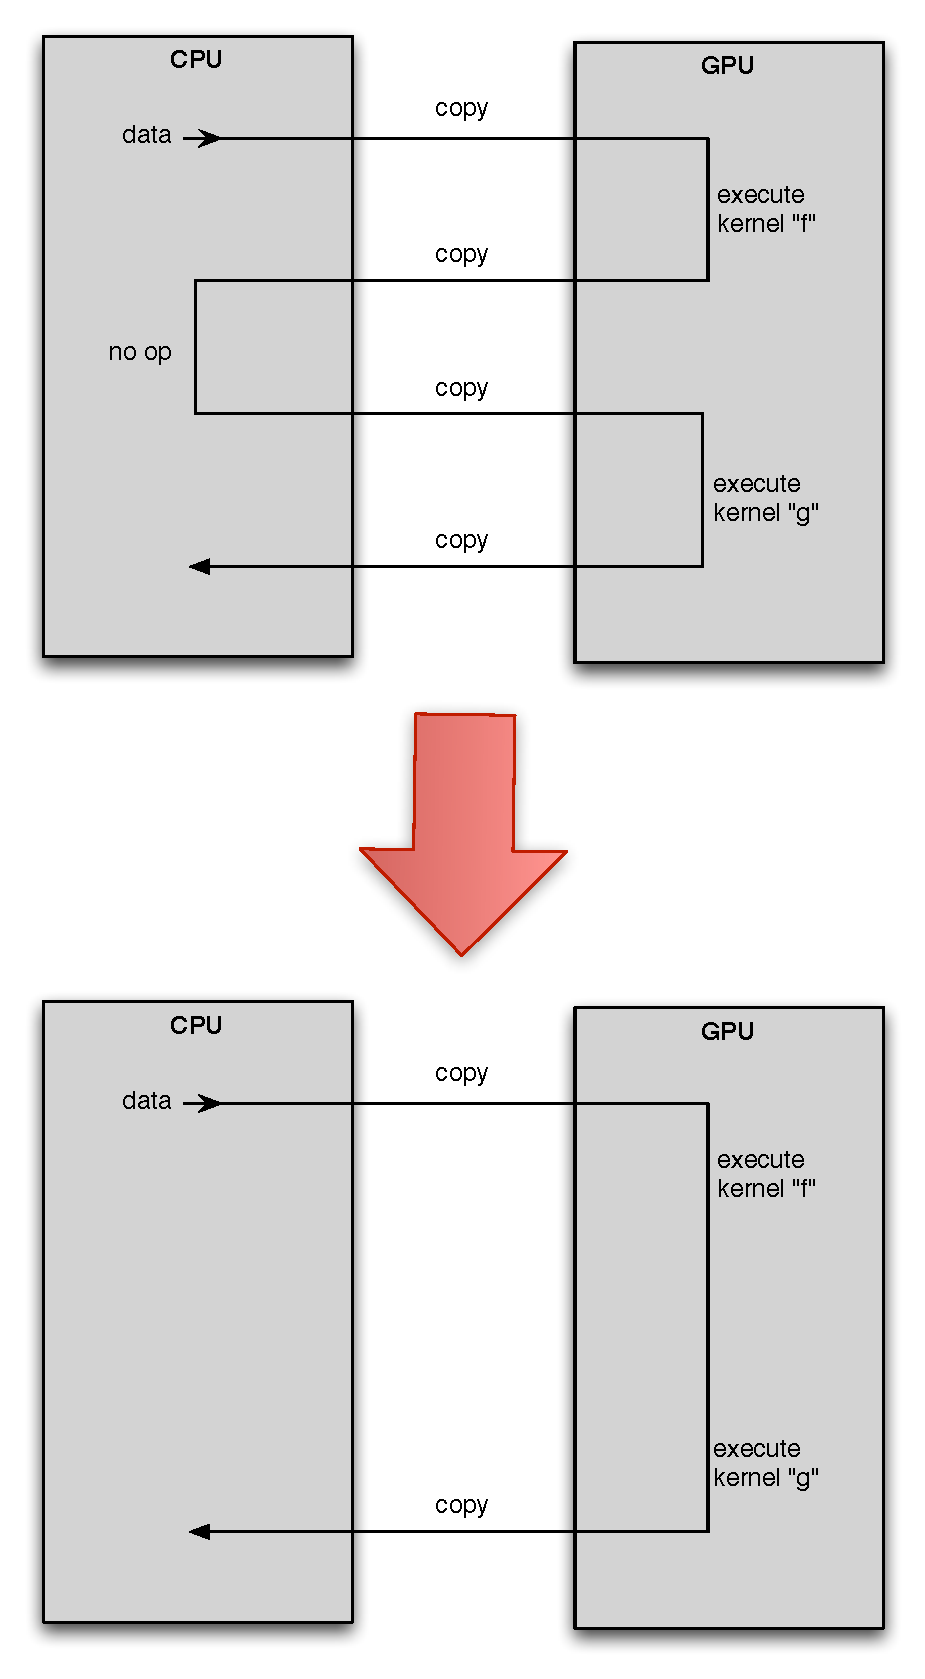
\includegraphics[width=1.8in]{images/basic-idea}
\caption{Elimination of redundant data copies}
\end{center}
\end{figure}

Twig operates on data types instead of data. The input to a Twig program is a
data type, and the output is a transformed data type along with some generated
code that will perform the transformation on data in the target language. For
this reason, Twig is restricted to operate only on types that can be represented
in the target language, (e.g., for C, things like \texttt{int}, \texttt{float},
or \texttt{structs}). It can, however, augment the information about those types
to make them more restrictive. For GPU programming, we exploit this capability
with the addition of \emph{located types}.

\subsection{Located Types}
\label{sec:located-types}

% An important principle of Twig's design is the ability to augment type
% information. Twig generates C code, and that code must therefore conforms to
% C's type system. However, Twig can operate on more complex types, as long as
% these types have a mapping to C. This enables us to design primitive rules
% that insist on stricter type information than would be available in C alone.

For GPU programming, we exploit Twig's augmented types by adding a notion of
\emph{location} to the usual C types. Location in this case describes where the
data is stored in memory, i.e., either in system memory or on the GPU.

For example, we can have an array of \texttt{int}s on the CPU (represented in
Twig as the type \texttt{array(int)}), or the same data type but located on the
GPU (represented as \texttt{gpu(array(int))}). This simple scheme allows one to
express transformations in Twig which take location into account explicitly.

By wrapping the basic data type with the location information, we ensure that
rules must be specific to the GPU in order to operate on GPU data. For example,
a rule

\begin{verbatim}
[gpu(array(float)) -> gpu(array(int))]
\end{verbatim}

promises to convert an array of floats to an array of integers, but only if the
data already resides on the GPU. If it does not, the data must be moved with a
rule such as

\begin{verbatim}
[array(float) -> gpu(array(float))]
\end{verbatim}

This simple but effective scheme enables facilitates automated reasoning about
the movement of data to and from the GPU.

Located types could easily be extended to support more complex location
information. For example, in a computer with multiple GPU devices, each device
could be assigned its own location.
